
\documentclass[draftclsnofoot,onecolumn,letterpaper,10pt,compsoc]{IEEEtran}
\usepackage[utf8]{inputenc}
\usepackage[margin=0.75in]{geometry}
\usepackage{listings}
\usepackage{graphicx}
\usepackage{color}
\usepackage{float}
\usepackage{subcaption}
\usepackage{filecontents}
\usepackage{lipsum}
\usepackage{hyperref}
\usepackage{verbatim}

\begin{document}
\begin{titlepage}
  \begin{center}
        \vspace*{1cm}
 
        \begin{center}
            \Large
            \textbf{Fortran to Python Conversion}
        \end{center}{}
     
        \vspace{0.2cm}
        Problem Statement\\
        \vspace{0.3cm}
        
        Brian Hambleton, Dakota Alton, Ian Band, Ivan Halim\\
        CS461 - Section 001 - Fall 2019\\
        Group 40
        
        \vspace{1.5cm}
        
        \begin{abstract}
        
            This paper outlines the problem in using legacy simulation software described by Genevieve Segol. As well, it outlines a solution for building a better, more portable, system for generating simulations of hydrologic system behaviors for use in water-resource research. The application will be developed to dynamically execute a numerical model estimating the behavior of groundwater. A modern graphical interface will be designed and developed to enhance both usability and portability of the application. This could facilitate a wider range of use for the model in other applications for hydrology research.

        \end{abstract}
        
        \vfill
        
        \vspace{0.8cm}
 
  \end{center}
\end{titlepage}

\tableofcontents

\newpage

\section{Introduction}
\subsection{Purpose}
This document defines the application Group40 will be developing as their Capstone project, identifies the requirements and the target audience for this application, and outlines the proposed approach.

\subsection{Product Overview}
Group40 will build an application to replace an outdated Fortran code. This application will be able to run on both desktop computers and laptops. 

\subsubsection{Product Functions}
The product is responsible for capture the behavior of two legacy Fortran simulations. The first simulation models groundwater flow and containment transportation in two dimensions. The second simulation models the same, but in three dimensions. We fill first implement the two dimensional model, and after completing this portion of the program we will move on to implementing the three dimensional calculations.

The product is also meant to expand on the utility of the legacy Fortran simulations. To do this, it we will convert the existing code base to Python and incorporate a graphical user interface. These actions are meant to accomplish two goals. The first goal is to allow the application to be run on a wider array of devices. The second goal is to improve user experience by including a graphical method for specifying inputs and viewing outputs. 

\subsubsection{User Characteristics}
The users of this application are professionals, working in the private or public sectors. For example, private sector professionals may be working for engineering and construction firms, and public sector professionals may be working for government agencies such as the Environmental Protection Agency. These professionals are typically familiar with using applications similar to what we will develop.

\subsubsection{Limitations}
\subsection{Definitions}
\begin{itemize}
    \item Graphical User Interface (GUI): Interface that visualizes actions that can be taken as well as give graphical feedback.
\end{itemize}

\section{Revision History}
\subsection{22 November 2019}
Modifications made to the sentence structure of 1.1, 1.2.1 and 1.2.2 based on client's recommendations. 
\subsection{3 December 2019}
Modifications made to content and structure of sections 3.2, 3.2.2, 3.3, and 4.1.
\section{References}

\section{Specific Requirements}

\subsection{External Interfaces}
For the external interface, we will be using a Python library called \textbf{PyQt}. This library will allow us to build a form that our users can fill out to specify the parameters of the simulation. The interface will also be responsible for sending the data to the backend as to visualize the simulations output. The interface will also have a dedicated section for documentation explaining what each parameter in a function is for, along with what the output represents.

\begin{figure}
\centering
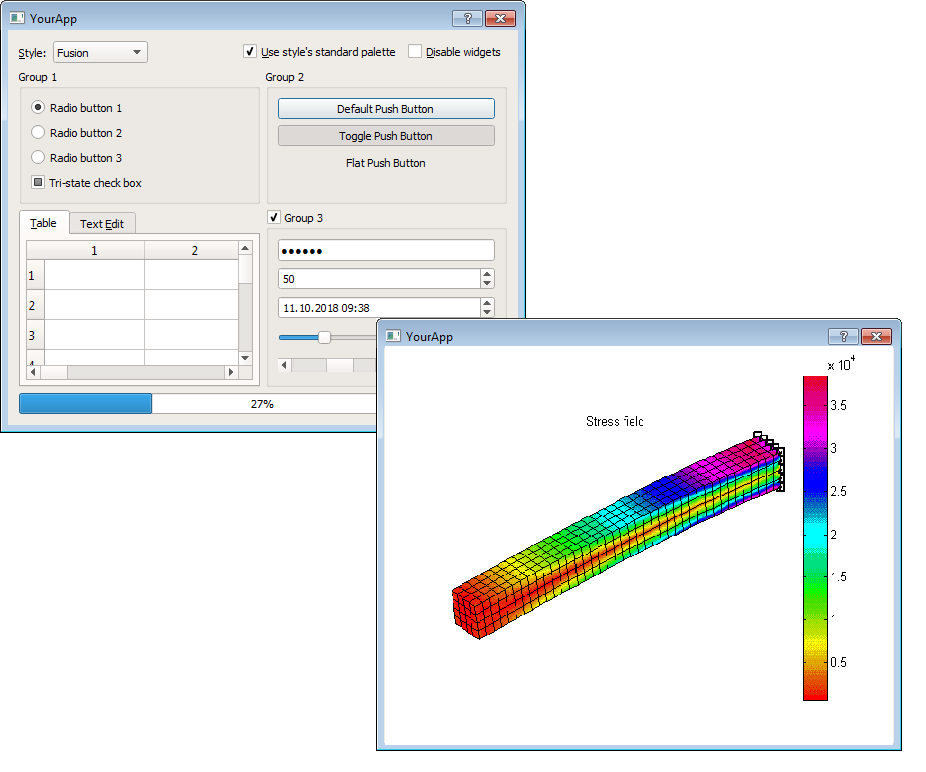
\includegraphics[scale=0.8]{form.png}
\caption{Sample form using PyQt.}
\label{fig:form}
\end{figure}

\subsection{Functional Requirements}
\subsubsection{Graphical User Interface}
The GUI will allow users to easily input and modify all variables required to run a simulation.

\subsubsection{Preparation of Finite Element Mesh}
\begin{itemize}
    \item The system must represent the flow region by a finite element mesh.
    \item The system must construct the mesh by dividing the flow region into elements.
    \item The mesh should identify important features such as interfaces between different materials, location of recharge or discharge, etc.
    \item The mesh should conform to the exterior boundaries of the flow region and to the interface between different materials.
    \item Nodes should be numbered sequentially along the shorter axis of the flow model (the one with the smaller number of nodes).
    \item Each element must be assigned a material number.
    \item Hydraulic and mass-transport properties must be specified for each material.
    \item For each node in the finite element mesh, x-coordinate, y-coordinate (z-coordinate for 3D), initial pressure head and initial concentration must be specified.
\end{itemize}

\subsubsection{Program Output}
\begin{itemize}
    \item A list of the input data including all nodal and element attributes.
    \item A list of the solution for the dependent variables (pressure and concentration) at the specified intervals.
    \item A graphical display of the results of the simulation. The display will be modifiable by the user.
\end{itemize}

\subsubsection{Error Message}
\begin{itemize}
    \item The variable ISTOP, initially set to zero, is used as an error indicator.
    \item If inconsistencies occur in the input data or during the assembly and solution processes, the value of ISTOP is increased by one and an error message is printed.
    \item Checks are performed regularly and if ISTOP is found to be nonzero the simulation is stopped.
    \item When the triangularization of the flow coefficient matrix fails, the row at which the triangularization failed is printed, the variable IEX is returned from DBAND with a value of one and execution is terminated.
\end{itemize}

\subsection{Usability Requirements}
It must be easy to learn how to use our groundwater simulation system. Otherwise, we cannot expect our users to switch to our system. In particular, success with the first attempt at obtaining a finite element mesh is important. Knowledge of Python will not be necessary for users to be able to create and run a simulation. Because of this the code must be well commented so any user with limited to no knowledge of Python will still be able to understand the code's functionality.


\noindent
To minimize user frustration, it is important that users understand the causes of errors.

\begin{itemize}
    \item When the system rejects an attempt: The system must display an error message explaining the cause of the error. In 90\% of such cases, the user must be able to understand the error message and be able to explain in his own terms what the cause is and what he can do about it. Examples: the input data is presented in the wrong format, the input value is invalid, the function call is missing an argument.
\end{itemize}

\subsection{Performance Requirements}
Because this program is going to be computationally heavy, the program must have at least 80\% of the performance of the original Fortran code. For data processing, calculation and finite-mesh generation, response times should be less than 2 seconds. Simulations should not take more than 5 seconds. Animations should reflect the given time-step.

\subsection{Logical Database Requirements}
The program does not require a database because input is supplied by the user through both the program's UI and a file(s) containing nodal information. Program output after the numerical simulation is completed will be displayed on the screen and provide users the option of saving to a file, no information will be stored in a database.

\subsection{Design Constraints}
Constraints for the program include file formatting and memory requirements. All user supplied data included in an input file will be required to adhere to a specific format to ensure data is interpreted by the program correctly.

\subsection{Software System Attributes}
\subsubsection{Reliability}
The system must be able to accurately perform calculations based on the user's input to create a simulation. This requires proper formatting of the user supplied file(s) to ensure the accuracy of the calculations. However if the file format is incorrect the program will throw an error specifying the incorrect format.

\subsubsection{Availability}
Because the program will be coded in Python, users will be able to execute the program on any system with a Python interpreter installed.

\subsubsection{Security}
The program does not require any sensitive information for input and its functionality is limited to performing calculations on user supplied numerical data so encrypting the data is not a necessary feature.

\subsubsection{Maintainability}
The program will be implemented with well modularized code that follows the Python Enhancement Proposal 8 (PEP 8) coding style. This results in readable code that will be easy to navigate to make any updates or modifications to the system.

\subsubsection{Portability}
The program's portability is the main purpose of this project and is why it will be implemented in Python. This allows the program to be run on any device with a Python interpreter and the necessary modules and libraries installed.

\subsection{Supporting Information}
\subsubsection{File Input Formatting}
This program will depend on user supplied information to specify the parameters for the underlying calculations the program will perform to develop a simulation. The user supplied information will include input  through the GUI, as well as coordinate plots supplied via a file. As a result a pre-determined formatting will be required for files and displayed to the user.

\section{Verification}
\subsection{External Interfaces}
To gain feedback on the usability of our program we will conduct user studies by allowing a small number of users to review the GUI and attempt to run a simulation. This will allow users to provide feedback on the system.

\subsection{Functional Requirements}
To ensure that functional requirements are met, we need 3 things: Unit testing, rapid prototyping and constant client interactions. Unit tests help us catch problems very early in the development process and keep us on track. Rapid prototyping helps us capture missed requirements through product validation by team members, client and users, thus reducing the risk of misunderstanding. Constant interaction with client helps us understand our client better and improves the chance that our software will meet our client’s needs.

\subsection{Usability Requirements}
Usability requirements are verified with this usability test: 10 test subjects with Python experience and 10 without Python experience are selected for interviews. In the interview, they try the two basic tasks and the tasks causing the system to reject the request for many different reasons. Task completion times are recorded manually. The percentages are interpreted relative to the sample of 10 persons. For example, 9 of the 10 users must be able to generate a finite element mesh within 5 minutes.

The performance for experienced users is verified in this way: 3 test subjects from each group are allowed to practice generating a finite element mesh six times. They are asked to come back three days later and perform the same task again. It is important that users get no other help than what they would get in a real-life situation.

\subsection{Performance Requirements}
The performance can be measured by performing a running time analysis on the Python code and the Fortran code. We will use the system clock to record the running times of each algorithm for ten different values of input size. The Python code is considered successful if it has the same time complexity as the Fortran code with increasing input size.

\subsection{Logical Database Requirements}
The program does not require a database and therefore does not require verification of database requirements.

\subsection{Design Constraints}
File formatting supplied by the user is the main design constraint of our program. Qualifying if these constraints have an impact on the usability of our program will be determined during user testing.

\subsection{Software System Attributes}
Verifying system attributes; reliability, availability, maintainability and portability will be done through user testing. Security is omitted because it is not included in our requirements based on the programs functionality.

\section{Appendices}
\subsection{Assumptions and Dependencies}
To make the application usable and accessible to users, we must make the assumption that they have limited knowledge of software and computers, and do not have a background in programming or computer science.

\subsection{Acronyms and Abbreviations}
\begin{itemize}
    \item GUI: Graphical User Interface
    \item UI: User Interface
    \item PEP: Python Enhancement Proposal 
    \item NumPy: Python Number Library
    \item SciPy: Python Science Library
    \item Plotly: Python Plotting Library
\end{itemize}
\pagebreak

\section{Gantt Chart}
\begin{figure}[htp]
    \centering
    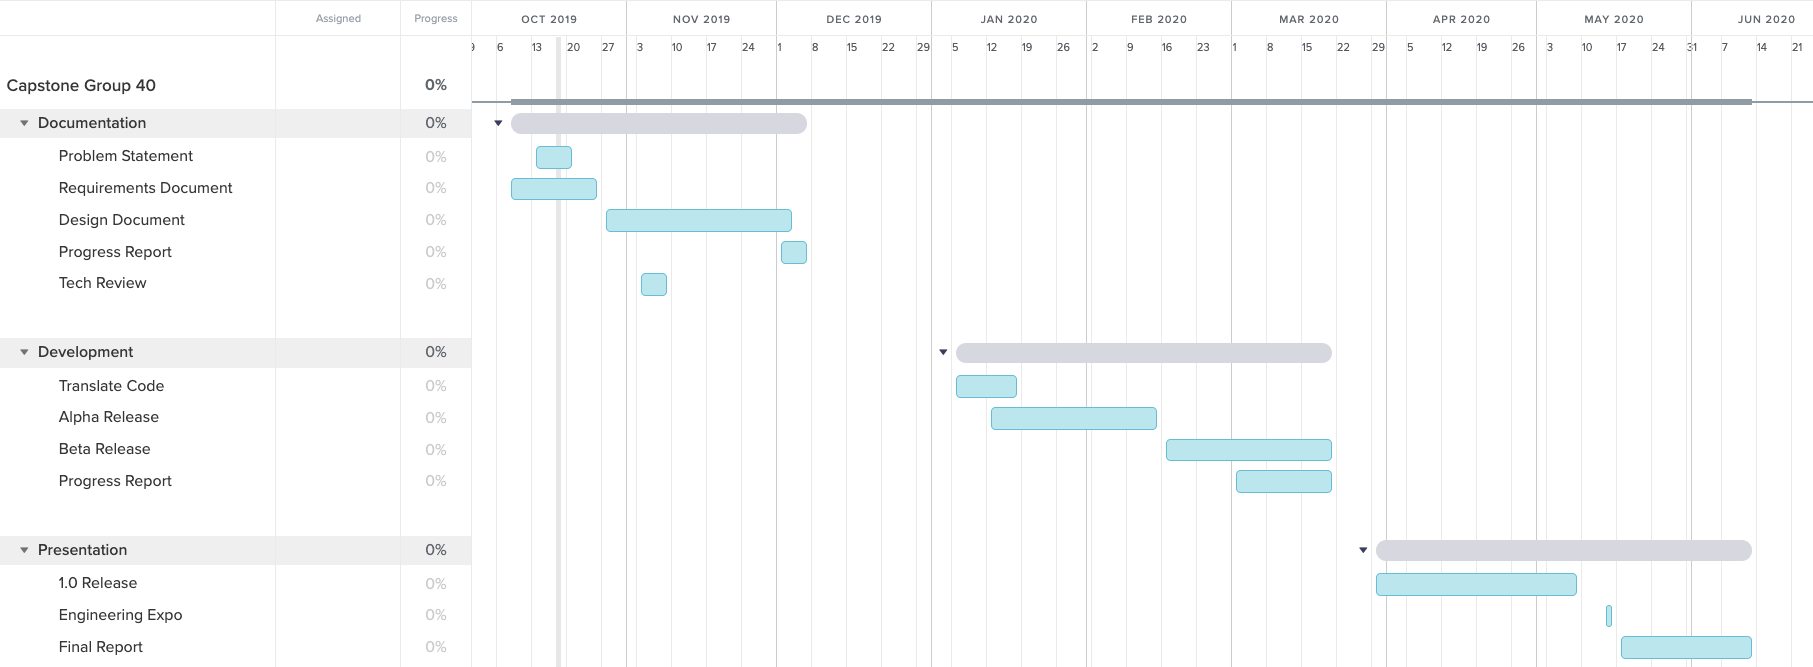
\includegraphics[width=17.5cm]{gantt-chart.png}
    \caption{Gantt Chart}
    \label{fig:galaxy}
\end{figure}



\end{document}